\section{Numerical Model Approach}
\label{sec:NumericalModelApproach}

\subsection{Workflow}
\label{subsec:SoftwareSetup}

\begin{figure}[h!]
    \centering
    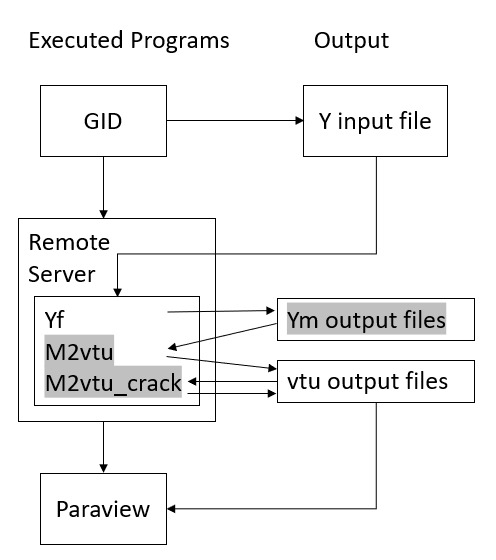
\includegraphics[width=\columnwidth]{Workflow}
    \caption{Workflow of generating a simulation}
    \label{fig:workflow}
\end{figure}

The workflow is illustrated in Fig. \ref{fig:workflow}. The grey shaded items are removed using this paper such that the \texttt{Yf} code now generates the \texttt{VTK} output files directly. The workflow was tested on \texttt{Ubuntu 18.04.2 LTS} subsystem for \texttt{windows 10}.

\bigbreak
A \texttt{2D} input \texttt{Y} file is generated on \texttt{Windows 10} using the open source pre-processor \texttt{CAD} software \texttt{GID} \cite{GID11}. It is possible to instead import the geometry from other \texttt{CAD} software, such as \texttt{AutoCAD}.

\bigbreak
The input file is compiled using three binary files \texttt{Yf}, \texttt{m2vtk} and \texttt{m2vtk\_crack}, which constitute the \texttt{Y2D} code. The program may be obtained from the \texttt{AMCG} at Imperial College London. Code execution requires obsolete \texttt{VTK 5.8} libraries and the obsolete operating system \texttt{Ubuntu 14.4}. Tests were conducted on two remote servers, the high performance computing (\texttt{HPC}) system at Imperial College and a private remote university server.

\bigbreak
The code outputs \texttt{.vtu} files which compose a time series simulation. The output is visualised using the open source software \texttt{Paraview}.

\subsection{Geometry Setup}
\label{subsec:GeometrySetup}

The input file contains the model including the geometry, constraints, materials, as well as the simulation parameters. The majority of modelling parameters are adduced from the literature. A list of material parameters is given in appendix table \ref{tab:matpar}. A list of input file simulation parameters is provided in appendix table \ref{tab:simpar}.

\begin{figure}[h!]
    \centering
    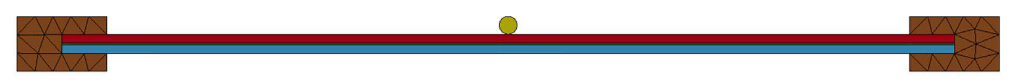
\includegraphics[width=\columnwidth]{Geometry}
    \caption{\texttt{2D} geometry of the laminated glass structure and projectile \cite{Che18}}
    \label{fig:geometry}
\end{figure}

Fig. \ref{fig:geometry} illustrates the \texttt{2D} geometric setup. The figure shows the initial state of the spherical projectile (yellow) immediately before impact on the laminated glass (impactor glass plies in red, inner glass ply in blue, inter-layer in green). The glass is fixed via a support system (brown). The support structure is not modelled for now and is replaced with no-velocity boundary conditions acting on the sides of the glass plies. 

\bigbreak
In real-world applications, the dimensions of the inter-layer are smaller compared to the glass plies. Therefore, a translational degree of freedom in the \texttt{y}-direction exists for the inter-layer. This effect will also need to be considered in this paper.

\bigbreak
Critical flaws, which cause complete structural failure, are usually found on the cut and machined glass edges \cite{Pel16}. Based on this consideration, the boundary structure layout requires special care. A project task remains to determine a realistic boundary structure to be applied.

\bigbreak
Modifications to this preliminary geometric setup will include changes to the shape of the projectile, as well as changes to the thickness of the layers. A potential consideration is to model the projectile as firearm ammunition instead of a circle (or sphere). A symmetry boundary condition may be applicable and only half of the laminate may need to be modeled.

\bigbreak
The dimensions of the glass plate is set to $2000\,{\rm{mm}}\times2000\,{\rm{mm}}$ in order to avoid anisotropic effects. The thickness of the glass plies is set to $2\,{\rm{mm}}$ and $0.76\,{\rm{mm}}$ for the inter-layer. For now, a \texttt{PVB} material is chosen for the inter-layer.

\bigbreak
The preliminary mesh for all bodies consists of triangular elements. For the \texttt{3D} model, tetrahedral elements \cite{Che18} are to be considered. The preliminary element size is $1\,{\rm{mm}}$. Necessary modifications include reducing the number of elements for the projectile, as it is not of interest for the analysis and increasing the element size for far-field mesh elements for the plies and inter-layer. Potentially, differently shaped elements are more optimal for the results. The glass and inter-layers need to consist of several element layers to enable a more precise analysis. 

\subsection{Material Parameters}
\label{subsec:MaterialParameters}

Table \ref{tab:matpar} lists the material parameters for glass, \texttt{PVB}, steel and rock. The literature provides values for most of the quantities, although they are extremely diverse in some cases. The values used in this paper are marked bold. The elastic and contact penalties are evaluated using Eq. \ref{eq:p}.

\begin{table*}
  \setlength{\tabcolsep}{2pt}
  \small
  %\flushleft
  \caption{List of Y2 input material parameter values.}
  \begin{tabular}{@{}lllll@{}}
    Property & Glass & PVB & Steel Projectile & Rock\tablefootnote{for reference}  \\\midrule
    
    Density $\rho\,\left[{\rm{kg}} / {\rm{m}}^3\right]$
    
                &$2500$ \cite{Xu10, Aba13, Che18, Ved17, Gao14}  
                
                &\begin{tabular}[t]{@{}l@{}}
                    $870$ \cite{Gao14} \\ 
                    $\bm{1100}$ \cite{Xu10, Che18, Ved17} \\
                    $1105{\rm{e}}3$ \cite{Che18}\\
                \end{tabular}
                
                & $7800$ \cite{Che18} & $2700$\\[1em]

    Young's Modulus $E\,\left[{\rm{Pa}}\right]$
    
                & \begin{tabular}[t]{@{}l@{}}
                    $\bm{7{\rm{e}}10}$ \cite{Xu10, Che18, Ved17}\\
                    $7.409{\rm{e}}10$ \cite{Gao14}\\
                    $7.41{\rm{e}}10$ \cite{Che18}\\
                    $7.5{\rm{e}}10$ \cite{Aba13}\\
                \end{tabular}
                
                & \begin{tabular}[t]{@{}l@{}}
                    $\bm{1{\rm{e}}8}$ \cite{Che18} \\
                    $2.2{\rm{e}}2$ \cite{Ved17}\\
                    $5{\rm{e}}10$ \cite{Gao14}\\
                \end{tabular}
                
                & $2{\rm{e}}11$ \cite{Che18} & $3{\rm{e}}10$ \\[1em]
                
    Poisson's Ratio $\nu$ & \begin{tabular}[t]{@{}l@{}}
                                $0.2$ \cite{Che18, Gao14} \\
                                $0.21$ \cite{Aba13} \\
                                $0.3$ \cite{Che18} \\
                                $0.22$ \cite{Xu10} \\
                                $\bm{0.23}$ \cite{Ved17}\\
                                $0.25$ \cite{Che18}
                            \end{tabular}
                          
                          & \begin{tabular}[t]{@{}l@{}}
                                $0.42$ \cite{Che18} \\
                                $0.45$ \cite{Aba13} \\
                                $0.48$ \cite{Gao14} \\
                                $0.49$ \cite{Che15} \\
                                $\bm{0.495}$ \cite{Ved17}
                            \end{tabular}
                          
                          & $0.29$ \cite{Che18} & $0.205$\\[1em]
                          
    Mass damping coefficient $\mu$\tablefootnote{Rayleigh damping, viscous damping} (see Eq. \ref{eq:massdamp}) & $0$ & $0$ & $0$ & $0$ \\[1em]
    
    Elastic penalty term (see Eq. \ref{eq:p}) & $7{\rm{e}}11$ & $1{\rm{e}}9$ & $2.0{\rm{e}}12$  & $3.0{\rm{e}}11$\\[1em]
    
    Contact penalty (see Eq. \ref{eq:p}) & $7{\rm{e}}11$ & $1{\rm{e}}9$ & $2.0{\rm{e}}12$  & $3.0{\rm{e}}11$\\[1em]

    Mode I energy rate $G_{\rm{I}}\,\left[{\rm{J}}/{\rm{m}}^2\right]$ & 
    
    \begin{tabular}[t]{@{}l@{}}
            $\bm{10}$ \cite{Xu10}\\
            $3.9$ \cite{Che18} \\
            $4.0$ \cite{Che18}
        \end{tabular}
        
    & \begin{tabular}[t]{@{}l@{}}
            $2.8{\rm{e}}3$ \cite{Hoo17} \\
            $\bm{20}$ \cite{Che18}
        \end{tabular}  
    
    & $1.9{\rm{e}}5$ \cite{Sta00} & $20.0$\\[1em]

    Mode II energy rate $G_{\rm{II}}\,\left[{\rm{J}}/{\rm{m}}^2\right]$ & $50$ \cite{Xu10} & $2.8{\rm{e}}3$ & $1.9{\rm{e}}5$ & $100.0$ \\[1em]
    
    Mode III energy rate $G_{\rm{III}}\,\left[{\rm{J}}/{\rm{m}}^2\right]$ & $50$ \cite{Xu10} & $2.8{\rm{e}}3$ & $1.9{\rm{e}}5$ & $100.0$ \\[1em]
    
    Tensile Strength $\sigma\,\left[{\rm{Pa}}\right]$ & \begin{tabular}[t]{@{}l@{}}
            $6{\rm{e}}7$ \cite{Che15}\\
            $3{\rm{e}}7$ \cite{Che18}\\
            $\bm{3.46{\rm{e}}7}$ \cite{Che18}\\
        \end{tabular}
        
        & \begin{tabular}[t]{@{}l@{}}
            $\bm{2{\rm{e}}7}$ \cite{Zan12}\\
            $1.862{\rm{e}}7$ \cite{Che18}\\
        \end{tabular}
        
        & $1{\rm{e}}7$ \cite{Wu14} & $4{\rm{e}}6$\\[1em]
        
    Shear Strength $\tau\,\left[{\rm{Pa}}\right]$ & $17.9$ \cite{Che18} & $17.9$ \cite{Che18} & & \\[1em]
    
    Internal friction coefficient $\eta$ (Eq. \ref{eq:intfriccoeff}) & $0.1$ \cite{Che15}  & $0.7$ \cite{Kun15} & $0.15$ \cite{Sah07} & $0.6$ \\[1em]
    
    Internal cohesion $c\,\left[{\rm{Pa}}\right]$ (Eq. \ref{eq:MohrCoulomb}) & $7{\rm{e}}10$ & $2.2{\rm{e}}2$ & $2{\rm{e}}11$ & $8{\rm{e}}6$ \\[1em]
    
    Pore fluid pressure\tablefootnote{\label{notrel}not relevant for glass, \texttt{PVB} and steel} $\left[{\rm{Pa}}\right]$ & $0$ & $0$ & $0$ & $0$ \\
    
    Joint friction coefficient\textsuperscript{\ref{notrel}} & $0.6$ & $0.6$ & $0.6$ & $0.6$ \\
    
    Joint roughness coefficient $\texttt{JRC}_{\rm{0}}$ \textsuperscript{\ref{notrel}, }\tablefootnote{\label{jrc}at laboratory conditions} & $15$ & $15$ & $15$ & $15$ \\
    
    Joint compressive strength $\texttt{JCS}_{\rm{0}}$\textsuperscript{\ref{notrel}, \ref{jrc}} $\left[{\rm{MPa}}\right]$ & $120$ & $120$ & $120$ & $120$ \\
    
    Joint sample size $\left[{\rm{m}}\right]$\textsuperscript{\ref{notrel}} & $0.2$ & $0.2$ & $0.2$ & $0.2$\\[1em]
    
    Interface friction & $0.1$ \cite{Che15} & $0.62$ \cite{Fah07} & $0.44$ \cite{Fah07} & $0.6$ \\
    
    2D Problems & plane strain & & \\\bottomrule
  \end{tabular}
  \label{tab:matpar}
\end{table*}

\subsection{Problem Parameters}
\label{subsec:ProblemParameters}

\begin{table}[t]
  \caption{List of Y2D input simulation parameter values.}
  \begin{tabularx}{\columnwidth}{ll}
    Parameter                               & Value                     \\\midrule
    Maximum number of timesteps $n_{\rm{t}}$ (Eq. \ref{eq:nt})& $2{\rm{e}}6$         \\
    Current number of timesteps             & $0$                       \\
    Restart file saving frequency           & $1{\rm{e}}2$              \\
    Gravity in \texttt{X} Direction (m/s2)  & $0$                       \\
    Gravity in \texttt{Y} Direction (m/s2)  & $0$                       \\
    Gravity in \texttt{Z} Direction (m/s2)  & $-9.8$                    \\
    Timestep (s) (Eq. \ref{eq:deltat})      & $1{\rm{e}}-6$             \\
    Output frequency                        & $2{\rm{e}}3$              \\
    Current number of iterations            & $0$                       \\
    Gravity setting stage (s)               & $0$                       \\
    Load ramping stage (s)                  & $0$                       \\
    Maximum dimension (m)                   & $10$                      \\
    Maximum force (N)                       & $1{\rm{e}}6$              \\
    Maximum velocity (m/s)                  & $100$                     \\
    Maximum stress (Pa)                     & $1{\rm{e}}8$              \\
    Maximum displacement (m)                & $0.1$                     \\
    Minimum joint aperture (m)              & $1{\rm{e}}-7$             \\
    Maximum contacting couples              & $1{\rm{e}}7$              \\
    Buffer Size $b$ for NBS (m) (Eq. \ref{eq:buff})& $7.60{\rm{e}}-5$       \\
    Accuracy (bit)                          & $32$                      \\
    Joint friction model                    & {\small Coulomb}          \\
    Initial aperture correlation            & {\small roughness}        \\\bottomrule
  \end{tabularx}
  \label{tab:simpar}
\end{table}

\begin{table}[t]
  \caption{List of auxiliary parameter values (to calculate simulation parameter values).}
  \begin{tabularx}{\columnwidth}{ll}
    Parameter                               & Value                     \\\midrule
    Total minimum element volume $V_{\rm{e}}$ ($m^3$)& $1.00{\rm{e}}-07$\\
    Total minimum edge $\Delta_{\rm{min}}$ (m)& $4.13{\rm{e}}-04$       \\
    Total real simulation time $t$ (s)        & $10$                    \\
    Critical time step glass (s) (Eq. \ref{eq:deltatcrit})& $2{\rm{e}}6$\\
    Critical time step steel (s) (Eq. \ref{eq:deltatcrit})&$2{\rm{e}}6$ \\
    Critical time step \texttt{PVB} (s) (Eq. \ref{eq:deltatcrit})&$2{\rm{e}}6$   \\
    Overall Mesh size (m)                   & $2.5{\rm{e}}-4$           \\
    Mesh size projectile (m)                & $2.5{\rm{e}}-4$           \\
    Mesh size plies (m)                     & $2.5{\rm{e}}-4$           \\
    Mesh size inter-layer (m)               & $2.5{\rm{e}}-4$           \\\bottomrule
  \end{tabularx}
  \label{tab:simpar}
\end{table}

\bigbreak
The radius of the steel sphere (or circle) is set to $2.5\,{\rm{mm}}$. The critical time step \cite{Far19}\footnote{\label{DEMPlus} for inquiries concerning this reference please contact the \texttt{AMCG} at Imperial College London} is set accordingly to

\begin{equation}
\label{eq:deltatcrit}
\Delta t_{\rm{crit}}=\sqrt{\frac{V_{\rm{e}}\footnotemark\,\rho\footnotemark}{p}}=\sqrt{\frac{0.000413\cdot7.8\cdot10^3}{4\cdot{10}^{11}}}{\rm{s}}\,.
\end{equation}

\addtocounter{footnote}{-2}
\stepcounter{footnote}
\footnotetext{volume  $\left({\rm{in}}\,{\rm{m}}^3\right)$ of the smallest finite element, without units}
\stepcounter{footnote}
\footnotetext{density $\left({\rm{in}}\,{\rm{kg}}/{\rm{m}}^3\right)$ of the material of the smallest finite element, without units}

The acceptable time step $\Delta t$ is given by

\begin{equation}
    \label{eq:deltat}
    \Delta t= \floor{\Delta t_{\rm{crit}}} = 3\rm{e}-6{\rm{s}}\,,
\end{equation},

where $\floor{\,}$ denotes the floor operator. To simulate real time $t=10\,{\rm{s}}$, the maximum number of time steps required \cite{Far19}\textsuperscript{\ref{DEMPlus}} is given by

\begin{equation}
    \label{eq:nt}
    n_{\rm{t}}=\frac{t}{\Delta t}=\frac{10\,{\rm{s}}}{3\,{\rm{e}}-6\,{\rm{s}}}=1{\rm{e}}6\,.
\end{equation}


\subsection{Verification}
\label{subsec:Verification}

Meeting specified accuracy standards \cite{Sto15} requires verification of the numerical model by use of data from numerical experiments. Physical experiments involving the breakage of glass by projectiles or shock blasts require special safety arrangements. Air blast impact experiments are being conducted outdoors by service company \texttt{Jabisupra} \cite{Jab16} in cooperation with Imperial College London. The company is active in the field of envelope security and specialises in protecting infrastructure from certain threats. The data from \texttt{Jabisupra} is not expected to yet be ready and applicable for this project. Many other researchers have already conducted impact experiments in the past and a majority of the findings from these experiments are likely to be applicable to verify the model for this project.

\bigbreak
Dynamic impact on laminated glass comprises hard and soft body impact \cite{Moh17}. Hard body impact such as ballistic impact \cite{Bra10} causes minimal deformation to the projectile, while soft body impact such as bird impact \cite{Moh17} causes the projectile to undergo extensive deformation.

\bigbreak
Relevant parameters of the impact projectile include the normal velocity \cite{Gra98, Kar14, Dar13, Wu14}, the mass \cite{Kar14, Dar13}, the angle \cite{Gra98, Kar14, Dar13}, the shape \cite{Dar13} and the size \cite{Wu14}. Relevant parameters for the outer glass ply include its dimensions \cite{Wan18}, its mass, the support conditions \cite{Wan18} and the make-up \cite{Wan18}. For the inter-layer, the material \cite{Moh18, Wan18, Mon04}, thickness \cite{Ji98, Kar14, Wan18} and temperature \cite{Moh18, Zha19} are relevant.

\bigbreak
Low velocity ($\approx 20\,\mathrm{m}/\mathrm{s}$) hard impact experiments include the use of projectiles in form of road construction chippings \cite{Gra98}, ballistics \cite{Mon04}, drop-down weights \cite{Che15, Mil12, Wan18}, aluminum projectiles \cite{Mil12} and steel balls \cite{Beh99, Flo98, Wan18}. High velocity (around $180\, {\rm{m}}/{\rm{s}}$) soft impact experiments include the use of silicon rubber projectiles \cite{Moh17} and gas guns \cite{Moh18}.

\bigbreak
Wang et al \cite{Wan18} found that the panel size had an inferior effect on the breakage resistance \cite{Wan18}. Similarly, Monteleone et al \cite{Mon04} found that only a local area of the ply around the impact absorbed the impact energy for high velocities.

\bigbreak
Karunarathna \cite{Kar14} found that impact velocity and plate thickness contributed significantly towards the impact resistance, compared to impact mass and inter-layer thickness. Wang et al \cite{Wan18} found an increased inter-layer thickness to have a negative effect on energy absorption. Liu et al \cite{Liu16} established that the inter-layer thickness did not contribute towards energy absorption. Behr and Kremer \cite{Beh99} found an increased inter-layer thickness to better protect the inner ply. Kim et al \cite{Kim16} numerically optimised the \texttt{PVB} inter-layer constitution to prevent all damage to the inner glass ply.

\bigbreak
Liu et al \cite{Liu16} numerically investigated the optimisability of the inter-layer in terms of energy absorption by simulating the impact of a human head. Zhang et al \cite{Zha19} investigated the influence of temperature on the inter-layer and found that a hybrid \texttt{TPU}/\texttt{SGP}/\texttt{TPU} inter-layer performed best over the entire range of tested temperatures.